\chapter{Software Project Design} 
% Main chapter title

\label{Chapter6} 
%Call reference to this chapter use \ref{ChapterX}

\lhead{Chapter 6. \emph{Software Project Design}} 
% Change X to a consecutive number; this is for the header on each page - perhaps a shortened title

\doublespacing
% LINE FORMATTING

%\clearpage
%\pagebreak

% MAIN SECTION ==============================
\section{Use-Case of project}

Below the use-case daigram shows the use-cases of the project.
\begin{figure}[H]
	\centering
	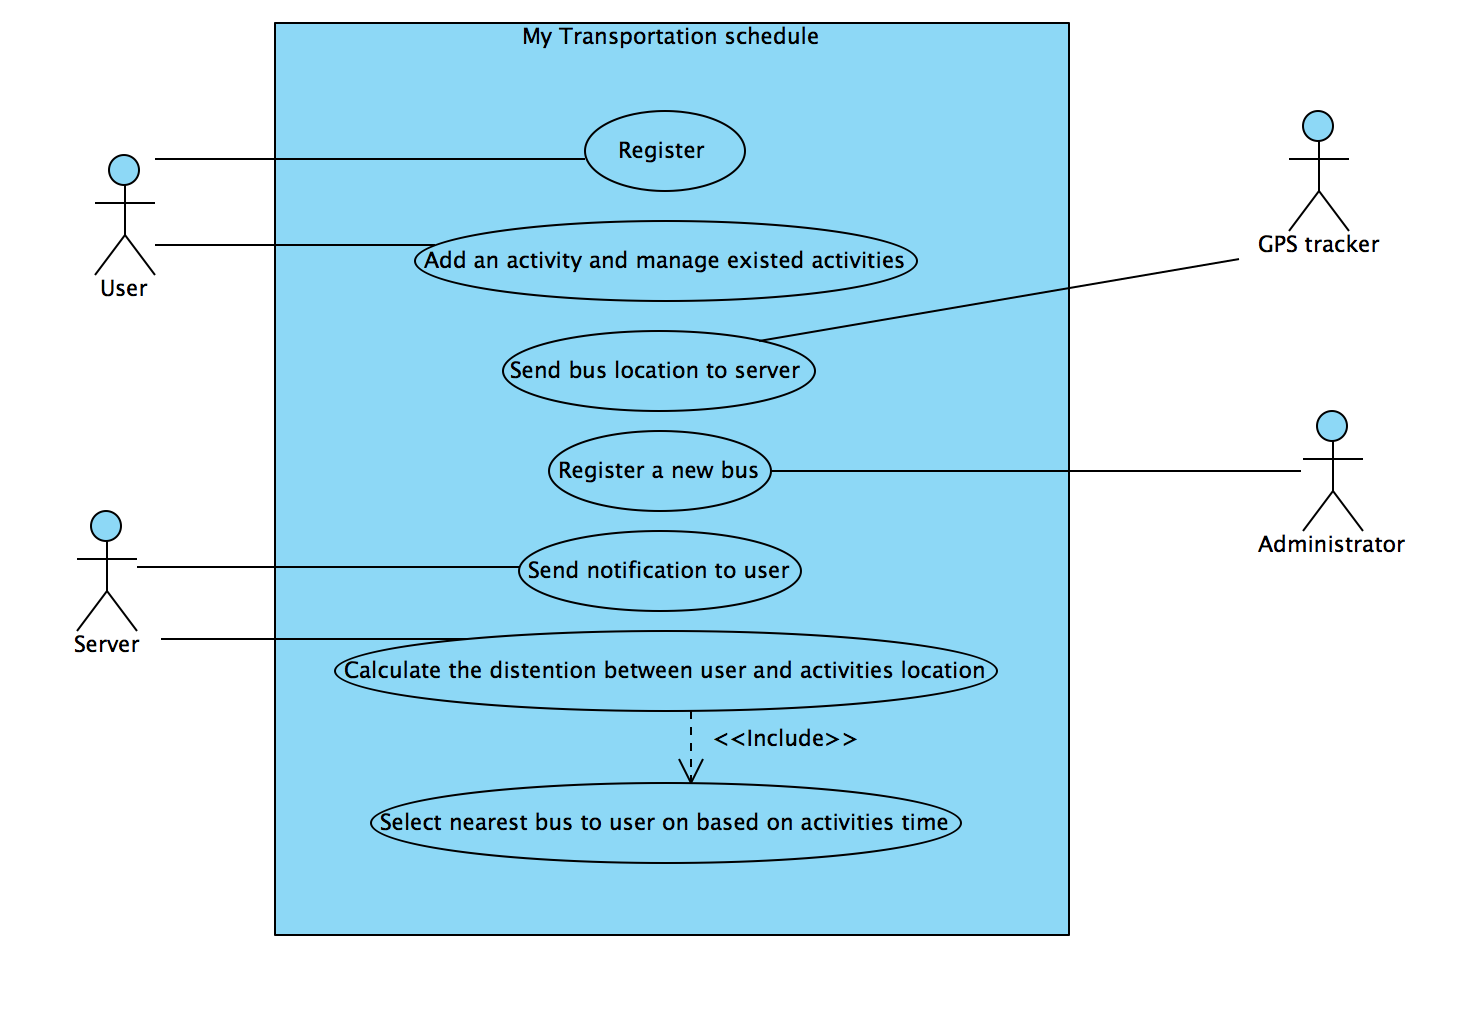
\includegraphics[scale=0.5]{Figures/FigureUseCase.png}
	\rule{35em}{0.5pt}
	\caption[Use-cases of the project]{Use-cases of the project}
\end{figure}

\section{Component Diagram}
Below is the Component Diagram shows the main software component and the interfaces between them.
\begin{figure}[H]
	\centering
	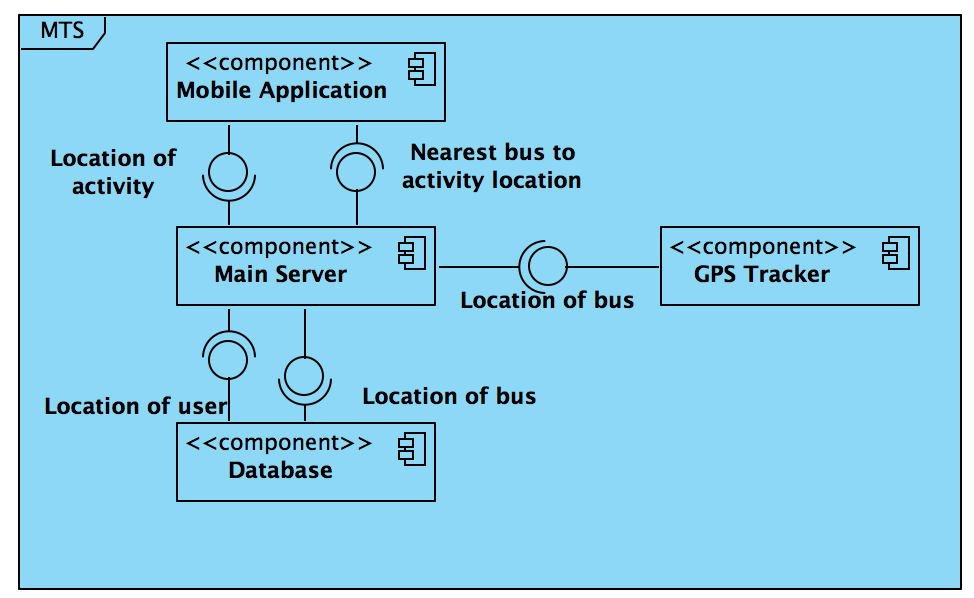
\includegraphics[scale=0.8]{Figures/FigureComponentDiagram.png}
	\rule{35em}{0.5pt}
	\caption[Component Diagram]{Component Diagram}
\end{figure}

\pagebreak
\section{Sequance Diagram}
Below is the Sequance Diagram shows the attraction between user and the software, and how the software works overall.

\begin{figure}[H]
	\centering
	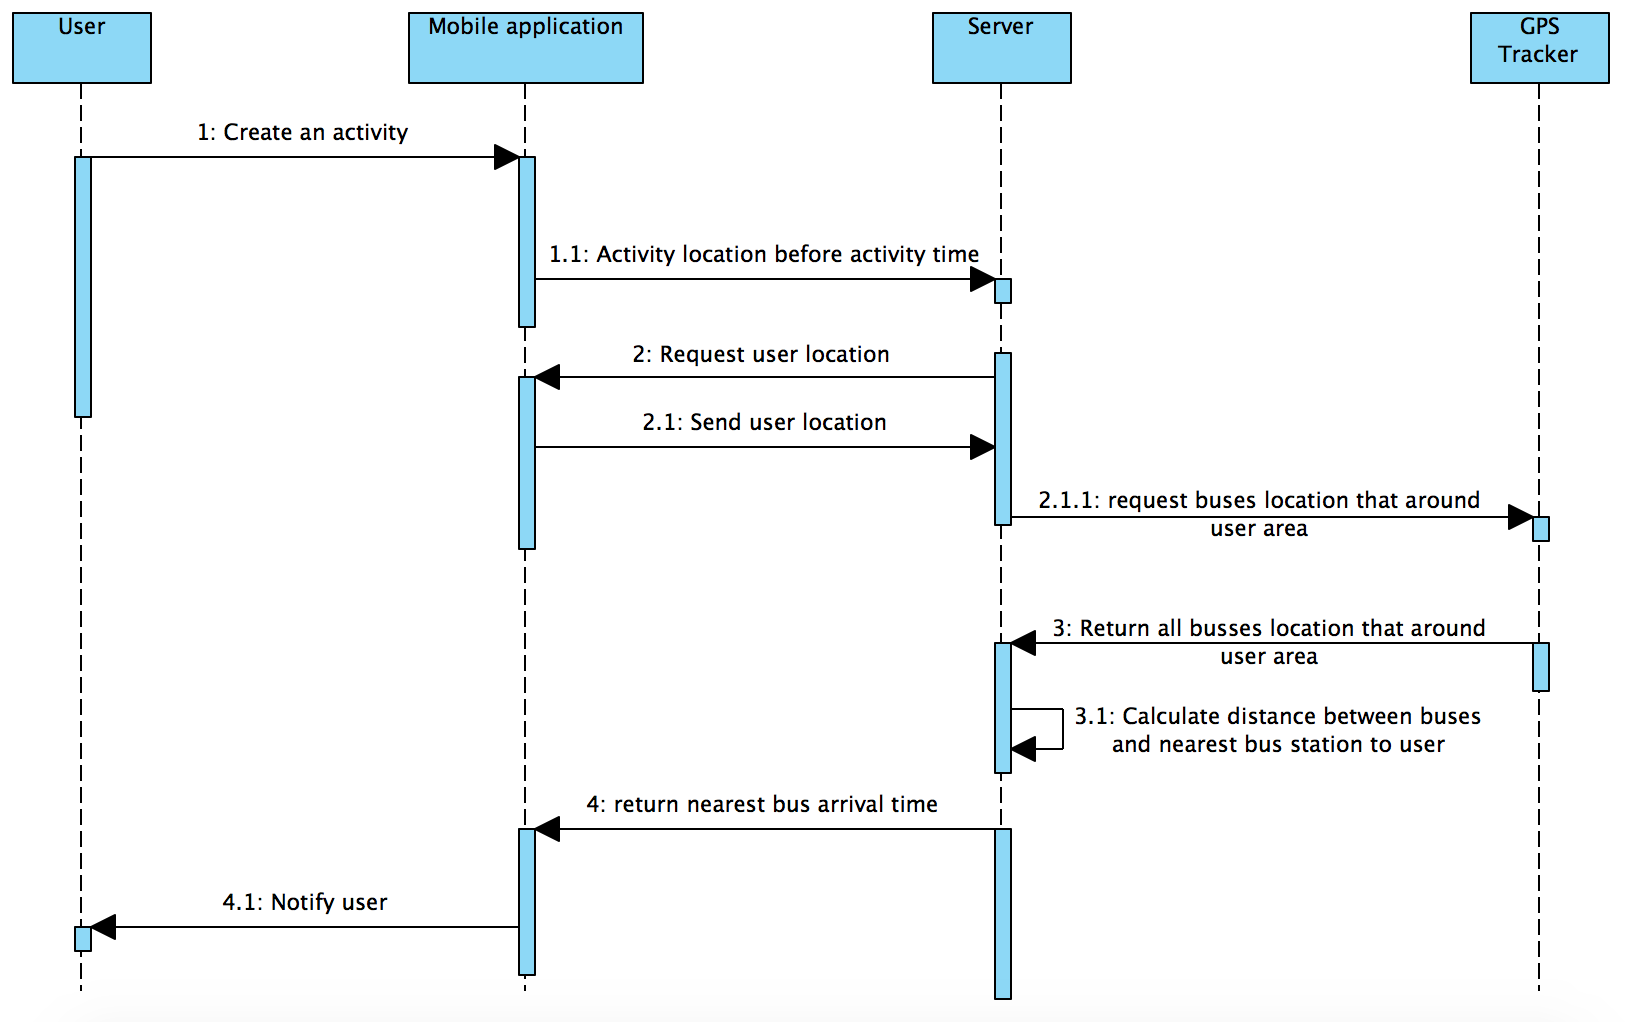
\includegraphics[scale=0.5]{Figures/FugreSequanceDiagram.png}
	\rule{35em}{0.5pt}
	\caption[Sequance Diagram]{Sequance Diagram}
\end{figure}
